\documentclass[a4paper]{article}

\usepackage[utf8]{inputenc}
\usepackage[polish]{babel}
\usepackage{polski}
\usepackage{listings}
\usepackage[T1]{fontenc}
\usepackage[margin=0.9in]{geometry}
\usepackage[usenames,dvipsnames]{xcolor}
\usepackage{lmodern}
\usepackage{pdfpages}
\usepackage{float}
\usepackage{longtable}
\usepackage{graphicx}
\usepackage{pdfpages}
\usepackage{multirow}

\begin{document}

\begin{titlepage}

\newcommand{\HRule}{\rule{\linewidth}{0.5mm}} 

\center 
 
%----------------------------------------------------------------------------------------
%	HEADING SECTIONS
%----------------------------------------------------------------------------------------

\textsc{\LARGE Politechnika Wrocławska}\\[1.0cm] % Name of your university/college
\textsc{\Large Bazy Danych}\\[0.2cm] % Minor heading such as course title
\textsc{\large Raport końcowy}\\[2cm]

%----------------------------------------------------------------------------------------
%	TITLE SECTION
%----------------------------------------------------------------------------------------

\HRule \\[0.4cm]
{ \huge \bfseries Analizator danych pogodowych}\\[0.4cm] % Title of your document
\HRule \\[3cm]
 
%----------------------------------------------------------------------------------------
%	AUTHOR SECTION
%----------------------------------------------------------------------------------------

\begin{minipage}{0.4\textwidth}
\begin{flushleft} \large
\emph{Autorzy:}\\
Aleksandra \textsc{Grzelak}\newline
Dorian \textsc{Janiak}\newline
Marcin \textsc{Ochman}

\end{flushleft}
\end{minipage}
~
\begin{minipage}{0.4\textwidth}
\begin{flushright} \large
\emph{Prowadzący:} \\
dr hab. inż. Grzegorz \textsc{Mzyk}
\end{flushright}
\end{minipage}\\[12cm]

{\large \today}\\[3cm] 


\vfill 

\end{titlepage}

\newpage
\tableofcontents
\listoffigures
\newpage

\section{Opis projektu}
W ramach projektu powstała baza danych zawierająca dane pomiarowe ze stacji pogodowych oraz interfejs graficzny w postaci strony internetowej. Do zrealizowania zadania posłużył serwer \textbf{MySQL} (przetrzymywanie oraz udostępnianie danych), język \textbf{Python} (logika aplikacji) wraz z modułem \textbf{Django} (framework web - strona graficzna oraz zarządzająca bazą). 
\section{Opis funkcjonalności}
Stworzony przez nas analizator realizuje poniżej wymienione funkcje:
\begin{itemize}
	\item \textbf{Wczytywanie danych pogodowych z plików CSV} - plik ma określony format (opisany w punkcie: 7.2). Funkcja uaktywnia się jedynie dla zalogowanych użytkowników aplikacji. Dostępna jest z poziomu panelu sterowania położonego w górnej części strony ("Wczytaj dane"). Wczytuje dane z pliku jednocześnie wpisując je do tabeli \verb Analyzer_danepomiarowe . 
	\item \textbf{Logowanie użytkownika} - logowanie odbywa się z poziomu górnego panelu sterowania ("zaloguj się"). Dane użytkownika domyślnie zapisane są w tabeli \verb auth_user . Jeśli wpisane hasło lub login nie pokryją się z zawartością bazy zostanie wyświetlony monit o niepoprawnym logowaniu. W przeciwnym wypadku logowanie przebiegnie pomyślnie i użytkownik otrzyma dostęp do funkcji wczytywania danych pogodowych. Została zaimplementowana również możliwość wylogowania użytkownika.
	\item \textbf{Rysowanie wykresów} - wykresy rysowane są gdy użytkownik wybierze jedną z opcji związaną z podglądem danych pogodowych. Do rysowania wykorzystywany jest pakiet \textbf{matplotlib}. Dzięki wykorzystaniu tej biblioteki stworzenie wykresu na stronie jest bardzo podobne do generowania wykresów w pakiecie Matlab.
	\item \textbf{Wybór stacji i rodzaju danych pomiarowych} - użytkownik wybiera stację oraz parametr, którego wykres chce wyświetlić. W programie po uruchomieniu funkcji reagującej na naciśnięcie odpowiedniego przycisku zostaje stworzony obiekt klasy Algorithm, który zawiera zestaw danych dla wybranej stacji oraz rodzaju pomiaru. 
	\item \textbf{Usuwanie danych pomiarowych} - jeśli użytkownik jest zalogowany ma możliwość z poziomu zakładki "podgląd stacji pogodowych" usunąć dane. 
	\item \textbf{Prognoza} - w programie został zaimplementowany algorytm prognozowania. Został on oparty na modelu \textbf{ARMA}. Algorytm nie jest jednak czystym prognozowaniem ARMA, został on zmodyfikowany. W naszej implementacji opiera się on również na interpolacji oraz wyznaczaniu wzmocnień.
\end{itemize}
\section{Opis tabel}
W raporcie opisujemy jedynie te tabele, które zostały utworzone bezpośrednio przez nas, ponieważ baza danych zawiera dodatkowo tabele, które tworzone są przez Django w momencie inicjalizacji projektu. Poniższa tabela zawiera pełne zestawienie pól stworzonych tabel.
W raporcie opisujemy jedynie te tabele, które zostały utworzone bezpośrednio przez nas, ponieważ baza danych zawiera dodatkowo tabele, które tworzone są przez Django w momencie inicjalizacji projektu.
Poniżej zamieszczony został diagram przedstawiający tabele i relacje między nimi:
\begin{figure}[H]
\centering
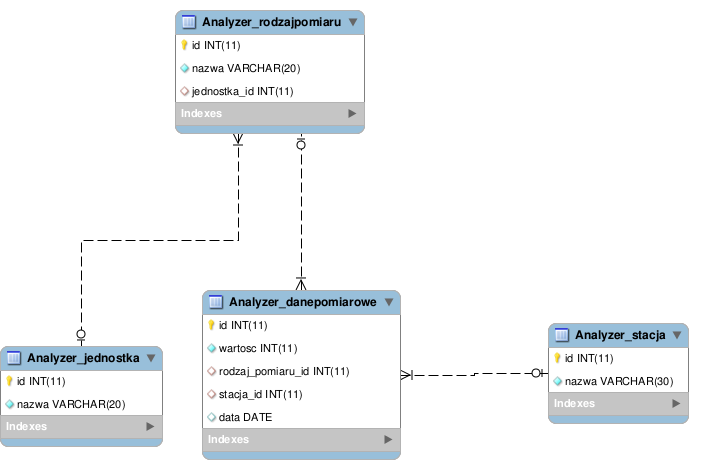
\includegraphics[width=\linewidth]{diagramEER}
\caption{Diagram tabel}
\label{fig:diagramTabel}
\end{figure}

 Poniższa tabela zawiera pełne zestawienie pól stworzonych tabel.
\begin{longtable}{|p{0.25\linewidth}|p{0.25\linewidth}||p{0.5\linewidth}|}
\hline
\textbf{Nazwa tabeli} & \textbf{Nazwa pola} & \textbf{Opis pola} \tabularnewline \hline \hline
\multirow{5}{*}{Analyzer\_danepomiarowe} & id & klucz główny (automatycznie inkrementowany) \tabularnewline\cline{2-3}
 & wartosc & całkowita część danej pomiarowej \tabularnewline\cline{2-3}
 & rodzaj\_pomiaru\_id & klucz obcy (tabela Analyzer\_rodzajpomiaru) \tabularnewline\cline{2-3}
 & stacja\_id & klucz obcy (tabela Analyzer\_stacja)\tabularnewline\cline{2-3}
 & data & data (godzina jest ignorowana) \tabularnewline\hline
\multirow{2}{*}{Analyzer\_jednostka} 
 & id & klucz główny (automatycznie inkrementowany) \tabularnewline\cline{2-3}
 & nazwa & jednostka pomiaru (np. C lub F dla temperatury) \tabularnewline\hline
\multirow{3}{*}{Analyzer\_rodzajpomiaru}
 & id & klucz główny (automatycznie inkrementowany) \tabularnewline\cline{2-3}
 & nazwa & nazwa rodzaju pomiaru, która będzie wykorzystywana do wyboru danych pomiarowych w aplikacji internetowej \tabularnewline\cline{2-3}
 & jednostka\_id & klucz obcy (tabela Analyzer\_jednostka \tabularnewline\hline
\multirow{2}{*}{Analyzer\_stacja}
 & id & klucz główny (automatycznie inkrementowany) \tabularnewline\cline{2-3}
 & nazwa & nazwa stacji, która będzie wykorzystywana do wyboru danych pomiarowych w aplikacji internetowej \tabularnewline\hline
\end{longtable}

\subsection{Opis tabel}
Tabele zostały specjalnie podzielone w taki sposób, aby móc w przyszłości łatwo dodawać kolejne wpisy. Poniżej krótko opisujemy stworzone tabele:
\begin{itemize}
	\item \textbf{Analyzer\_danepomiarowe} - w tabeli tej znajduje się pełne zestawienie danych pomiarowych. Dzięki wykorzystaniu kluczów obcych \textit{ rodzaj\_pomiaru\_id} oraz \textit{stacja\_id} można potem z tabeli filtrować potrzebne dane. Ponieważ w projekcie skupiliśmy się na pomiarach temperatury pole \textit{wartosc} reprezentowane jest przez liczbę całkowitą INT ze znakiem. Kolumna \textit{data} musi zawierać datę wykonania pomiaru, może również być w niej zapisana godzina, aczkolwiek zostanie ona w naszym programie zignorowana. W tej sytuacji można zauważyć, że domyślnie w naszej tabeli znajdują się daty w stylu \verb 2013-12-01  \verb 00:00:00  - godzina wynosi 0. Założyliśmy, że nie będą potrzebne nam pomiary z rozdzielczością godzinową.
	\item \textbf{Analyzer\_jednostka} - jednostka pomiaru została specjalnie wydzielona do osobnej tabeli, ponieważ w bazie może zdarzyć się sytuacja gdy przykładowo stworzony zostanie rodzaj pomiaru TMIN (temperatura minimalna) oraz TMAX (temperatura maksymalna), które mimo, że są różnymi rodzajami pomiaru, posiadają taką samą jednostkę - stopnie Celsjusza. Jednostka może zostać zapisana w maksymalnie 20 znakach, co oczywiście w takim wypadku jest bardzo dużym zapasem. Ponieważ jednostek w przypadku pogody nie będzie dużo nie należy przejmować się, że taka długość napisu może zająć zbyt dużo pamięci w bazie. 
	\item \textbf{Analyzer\_rodzajpomiaru} - rodzajami pomiaru mogą być np. temperatura, ciśnienie, szybkość wiatru itd. Nazwa, która zostanie wpisana w kolumnie \textit{nazwa} będzie widoczna później w aplikacji web. Z tego powodu można wpisać w jej ramach do 20 znaków. Rodzaj pomiaru powiązany jest kluczem obcym z jednostką. Później jest wykorzystywany przy wczytywaniu danych z pliku CSV.
	\item \textbf{Analyzer\_stacja} - tabela przechowuje poza kluczem głównym jedynie nazwy poszczególnych stacji. Na nazwę przyjęliśmy typ VARCHAR(30), czyli może składać się maksymalnie z 30 znaków. Nazwa stacji jest widoczna w aplikacji webowej oraz jest istotna przy wczytywaniu danych z pliku CSV.
\end{itemize}




\section{Użytkownicy}
cosikowo
\section{Sprawozdanie z implementacji i dokumentacji}
cosikowo
\section{Interfejs}
cosikowo
\section{Instrukcja obsługi}
\subsection{Instalacja bazy danych}
Baza danych została wdrożona na systemie Linux (przetestowana na dystrybucjach Ubuntu oraz Mint). Aby móc ją uruchomić należy wcześniej zainstalować poniższe pakiety:
\begin{itemize}
	\item python2.7
	\item python-numpy
	\item python-scipy
	\item python-matplotlib
	\item ipython
	\item ipython-notebook
	\item python-pandas
	\item python-sympy
	\item python-nose
	\item python-statsmodels
	\item python-tk
	\item mysql-connector-python
	\item django-pandas
	\item django-model-utils
	\item scipy
	\item mysql-server
\end{itemize}
Następnie koniecznie należy zaimportować bazę danych poprzez wywołanie poniższej komendy w terminalu w folderze głównym aplikacji (zawierający plik requirements.txt oraz manage.py):
\begin{verbatim}
	python2 manage.py migrate
\end{verbatim}

\subsection{Przygotowanie plików wejściowych}
Ponieważ aplikacja webowa nie pobiera sama danych pogodowych z internetu, należy je załadować z pliku. Aby móc to zrobić trzeba przygotować plik CSV zawierający komplet wymaganych informacji.
W kolejnych wierszach pliku muszą się znaleźć kolejne pomiary. W kolejnych wierszach należy pola oddzielić przecinkami:
	\begin{verbatim}
		nazwa_stacji,data_RRRRMMDD,rodzaj_pomiaru,wartosc_pomiaru
	\end{verbatim}
W przypadku pola \verb data_RRRRMMDD  data musi zostać zapisana w postaci ciągu cyfr nieoddzielonych żadnymi separatorami. Przykładowa zawartość pliku:
	\begin{verbatim}
		Warszawa,20130118,TMIN,-6
		Warszawa,20130119,TMIN,-8
		Warszawa,20130120,TMIN,-6
		Warszawa,20130121,TMIN,-7
	\end{verbatim}

Następnie należy ręcznie zarejestrować rodzaj pomiaru. Zostało to pozostawione stronie administracyjnej, ponieważ wiąże się to bezpośrednio z początkowym wdrażaniem bazy na serwerze. 
W tym celu należy dodać wpisy w odpowiednich tabelach:
\begin{itemize}
	\item \textbf{Analyzer\_jednostka} - dodać opis słowny i ID jednostki związanej z mierzoną cechą
	\item \textbf{Analyzer\_rodzajpomiaru} - dodać opis słowny zgodny z polem \verb rodzaj_pomiaru  z pliku CSV, nadać numer ID oraz odwołać się do klucza wpisanej przed chwilą jednostki
	\item \textbf{Analyzer\_stacja} - dodać nazwę stacji zgodnie z polem \verb nazwa_stacji  z pliku CSV oraz nadać jej numer ID.
\end{itemize}

\subsection{Pierwsze uruchomienie bazy}
Skonfigurowana baza danych wymaga jedynie uruchomienia środowiska, w którym będzie działać aplikacja internetowa. 
W tym celu (przy założeniu, że wszystkie zależności zostały wcześniej zainstalowane) należy stworzyć środowisko:
\begin{verbatim}
	virtualenv --no-site-packages env
	source env/bin/activate
	pip2 install -r requirements.txt --allow-external mysql-connector-python pandas scipy statsmodels django-pandas django-model-utils
\end{verbatim}
Aby uruchomić teraz bazę danych wystarczy:
\begin{verbatim}
	python2 manage.py runserver
\end{verbatim}
I następnie podany w konsoli adres strony skopiować i wkleić w przeglądarce internetowej (domyślnie: \verb http://127.0.0.1:8000/ ).

\subsection{Kolejne uruchomienie bazy}
Przy każdym kolejnym uruchomieniu bazy wystarczy ponownie uruchomić środowisko i serwer:
\begin{verbatim}
	source env/bin/activate
	python2 manage.py runserver
\end{verbatim}
oraz znowu skopiować adres i wkleić go do przeglądarki internetowej. 




\end{document}
